\documentclass{article}
\usepackage{parskip}
\usepackage{listings}
\usepackage{pdfpages}
\usepackage{amsmath}
\usepackage[margin=.6in]{geometry}
\begin{document}
\includepdf[pages=5]{Module5}
Comes from greek for secret writing. Cryptography is just making a plaintext message secret. Cryptography is a part of Cryptology which also includes cryptoanalysis which is when we try to do the reverse.
	
\includepdf[pages=7]{Module5}
We standardize our fictional characters. 
\begin{itemize}
	\item Alice, Bob, Carol, Dave - good honest hacker
	\item Eve - a passive eavesdropper that can't do anything
	\item Mallory - man in the middle
	\item Trent - trusted third party
\end{itemize}

\includepdf[pages=8]{Module5}
Confidentiality means we want to prevent Even from reading Alice's messages. We can do this using a cryptosystem

Integrity says we want to prevent Mallory from modifying Alice's messages. We can do this through message authentication (MACs), signature schemes, or cryptographic hash functions (not very secure since hackers can do this easily).

Privacy says we want to prevent MAllory from impersonating Alice. We can do this by passwords or biometrics and such, or through challenge response protocols.

A secret-key system or a public-key system. With a public key system we have two keys. A public key that anyone can use to encrypt something, and a secret private key that can be used to decrypt stuff. A secret key system can be block (requiring data to be a fixed width) or stream.


\includepdf[pages=9]{Module5}
We should only ever rely on a simple secret key that is easy to change. We could have a bunch of different encryption functions. This is not always practical so we encrypt with a long key that varies each time. A system is only as secure as the possible number of keys (we want the widest variety of keys to prevent brute forcing). Even then it is always possible to brute force no matter how long your key is. 

\includepdf[pages=10]{Module5}
A \textbf{strong crypto system} is one where iterating through every possible key is the best possible attack. 

\includepdf[pages=11]{Module5}
Frequently the attacker can get a small bit of plaintext from cypher text. For instance HTTP headers tend to be fairly standard so intercepting an encrypted request allows you to figure out a little bit. Breaking the enigma machine was done by getting a bunch of plaintext cyphertext pairs and analyzing them for a bit before breaking the code. To get these plain/cypher pairs they listened to this one base in russia that would send the same message every day (``weather report: all clear''). 

\includepdf[pages=13-19]{Module5}
A guy came up with pgp which allowed any key length. He ended up getting sued by the US government because encryption was classified as munition.

\includepdf[pages=20]{Module5}
A comity came up with the stupid number of 56 because the government wanted 48 so that they could break it with super computers but people wanted 64 so it would be more secure, so they split the difference.

\includepdf[pages=21]{Module5}
People wanted to show that DES was not all that secure so they held a contest for people to try to break it. Eventually the Electronic Frontier Foundation did it using a special machine. It took about 2 days to crack a key. Researchers eventually maked a system called copacobana that used fpgas (120, cost 10k) that could crack DES in about a week.

\includepdf[pages=22]{Module5}
Nowadays we use 128 bits. This is so huge that you cannot brute force attack it. So if the encryption is secure it is ``unhackable''. That being said, computers are continually getting faster by moore's law. So in 132 years you can break it in a day.

\includepdf[pages=23]{Module5}
\includepdf[pages=24]{Module5}
\includepdf[pages=25]{Module5}
\includepdf[pages=26]{Module5}
\includepdf[pages=27]{Module5}
RC4 is the most commonly used stream cipher, but it has a ton of problems (new hacks every year).

\includepdf[pages=28]{Module5}
Stream ciphers use the $\otimes$ operator since computers are super fast at them. They work using salts, but you have to be very sure that the salts are unique. Take you plaintext, $\otimes$ with key and add the salt. The encrypted text is sent along with the salt. Important to note, the salt is public knowledge.

\includepdf[pages=29]{Module5}
If we know the location in the string of the value you want to fuck with you can flip bits and such to change that number.

Most block ciphers (including AES) are based on substitution-permutation networks. They repeat their encoding steps a number of times around and around.
\begin{enumerate}
	\item $\otimes$ key bit state
	\item apply s-boxes (substitution box) which just takes a box of data and map it to something else (usually every 4 bits)
	\item permute bits
\end{enumerate}

At some point it was revealed that by switching to using the NSA's sbox mapping DES became more resistant to attacks around sboxes. This showed that they were about 10 years ahead of academic researchers.

\includepdf[pages=30]{Module5}
We have a block of plaintext, put it through cipher and get garbled mess. Problem arises when the block of plaintext is not the correct length (block must be multiple of some number). 

\includepdf[pages=31]{Module5}
Take your message and break it up into a bunch of fixed widths and just encrypt each one. This isn't that good because if any of those blocks are the same they will be encrypted the same. These patterns will appear in the encrypted text giving away more information than was intended. Think of a black and white image.

Never use ECB mode for encryption because it does this.

\includepdf[pages=32]{Module5}
A solution for this is to make each chunk dependent on the other chunks. Take the cipher text from the previous block and and it with the key for the next block to use as the key for that block. The message becomes a block longer because you need some starting cipher text to include.

\includepdf[pages=33]{Module5}
There is a ton of key information flying around so we need a good way to get it to the people who need them.

\includepdf[pages=35]{Module5}
\includepdf[pages=36]{Module5}
One key lets you encrypt and a different one lets you decrypt. An example is RSA. Public key = everyone knows it, secret key = no one knows it

\includepdf[pages=37]{Module5}
This is hackable if Mallory publishes a key to Alice to replace Bob's key with her own. When Alice looks up a public key Mallory replaces the encryption key with her own. Then she knows the decryption key so she can just listen in on the conversation. 

RSA was published in 1977 by Clifford Cox. It works by generating two large prime numbers, p and q that are inverses of eachother. So n = pq and ab=1 mod(p-1)(q-1). The public key is then (n, a) and the private key is (p,q,b). Encryption is $x^a mod n$ and decryption is $x^b mod n$. You want these numbers to be huge, but this makes doing the calculations very slow.

It is important that these are prime numbers else you could just factor the modulus.

\includepdf[pages=38]{Module5}
Public key systems have to have very large keys because people know them.

\includepdf[pages=39]{Module5}
To have equivalent security parameters the public key crypto will take 3 orders of magnitude more time to encryption than a symmetric crypto system.

\includepdf[pages=40]{Module5}
To get the best of both worlds we combine symmetric and public encryption. Say we have some plain text P that is a very long message. We generate an AES key called the session key. We get cipher text C by encrypting P using the session key. We then encrypt the session key using Bob's public key  using a public key system like RSA. 

\includepdf[pages=41]{Module5}
We still run into integrity problems. Just because it is secure does not mean that the message contents have not been altered in path.

\includepdf[pages=43]{Module5}

\includepdf[pages=44]{Module5}
Checksums are usually very simple so they really only work for accidentally errors, most attackers will just compute the checksum and set it properly,

Hash functions are nice because they don't have any key at all.

Authentication codes (mentioned earlier as MACs) have a shared secret key.

Signature schemes have a private signing algorithm and a public verification algorithm.

\includepdf[pages=45]{Module5}
MD5 is shit, do not use.

SHA is a set of standards published that hash algorithms should follow. Currently there have been no fully breaking attacks on SHA-1 just weakening ones, we want to all be moving to SHA-3.

\textbf{Preimage resistance} you should not be able to find any input that gives this output.

\textbf{Second preimage resistance} you should not be able to find another input that gives this output

\textbf{Collision resistance} you shouldn't be able to find an input or its output

We really want to make is so that hackers cannot find any collisions (when we accomplish this it is a strong hash function).


\includepdf[pages=46]{Module5}
Preimage resistance has us think of a bunch of inputs and try to get the given output of y (do the same for second preimage). Collision resistance is much easier since you just want to see if any two inputs have matching outputs, so it takes a square root number of times that preimage checks need.

\paragraph{Birthday Paradox} % (fold)
\label{par:birthday_paradox}
The odds of two people sharing a birthday in a room are significantly higher than the odds of someone in the room having the same birthday as me. This only takes roughly 23 people to get 50\% probability of two sharing a birthday.
% paragraph birthday_paradox (end)

You can weaken these hashes if they preserver character frequencies. 

\includepdf[pages=46]{Module5}
Currently this does not preserve integrity because Mallory knows the hash function so she can just rewrite the message, hash it, and swap thatin.

\includepdf[pages=47]{Module5}
\includepdf[pages=48]{Module5}
So hash functions are only good for preserving integrity when they cannot be messed with. 

\includepdf[pages=50]{Module5}
When we encrypt the message we take the last block of cipher text and that becomes the MAC

\textbf{HMAC} returns the hash of (key $\otimes$ opad append hash of (key $\otimes$ ipad append message)). opad and ipad are fixed public settings.

\includepdf[pages=51]{Module5}
Alice wantes to get message to Bob so she sends it using the shared secret key k. Alice also sends him the MAC of the message, from this Bob calculates the MAC of the message that Alice sent him and checks that this matches the MAC she sent him. Because the MAC calculation requires knowledge of the secret key you can use this to ensure integrity.

\includepdf[pages=52]{Module5}
\textbf{Encrypt then MAC} You can encrypt the message first and then MAC it, return encrypt(message) append MAC(encrypt(message))

\textbf{MAC then encrypt} encrypt(message append MAC(message))

\textbf{encryot and MAC} encrypt(message) append MAC(message)

Encrypt then MAC is the best of the options.

\includepdf[pages=53]{Module5}
\includepdf[pages=54]{Module5}
\includepdf[pages=55]{Module5}
Digital signatures are used when we don't want repudiation. It works using a public key system where the key is separated into two parts, a public and a private key.

\includepdf[pages=56]{Module5}
private key = signing

public key = verification

The private key is not for decryption, it is for signing things. So Alice privately signs the document and Bob can use the public key to verify the signature.

\includepdf[pages=57]{Module5}
Alice puts her secret key into some signing algorithm that also takes the message in. It outputs the signature that goes to Bob. Bob then uses the public validation key into a validation algorithm along with the signature which returns true or false if Alice is valid.

\begin{align*}
ab &= 1 \% (p-1)(q-1)\\
S &= M^b \% n\\
V &= S^a == M \% n\\
\end{align*}
S = signature, V = is valid, M = message, b = secret key, a = public key, n = private key * public key, p and q are large prime numbers


Its very tempting to think that signing is decryption and verification is encryption because they work similarly, but they are different. There is a tone of nuance that happens in actual signing schemes to make them secure which is what makes it different from en/decryption. The textbook gets this wrong, ignore the textbook.

DSA and ECDSA are the most commonly used signature schemes. DSA is messy to talk about so we are going to look at its precursor El gammal (this let to Schnorr  which led to DSA).

p = some large prime

$\alpha$ = generator for random int

$\beta = \alpha^a \% p$

the combination of p, $\alpha$, and $\beta$ are the public key and a is the private key.

\begin{align*} 
	Sign_k(M) &= (\gamma, \delta)\\
	\gamma &= \alpha^r \% p\\
	\delta &= (M-a\gamma)r^{-1} \% (p-1)\\
	(\gamma, \delta) &-\rightarrow Bob\\
	Ver_k(M,\gamma, \delta)) &= \beta^\gamma \gamma^\delta == \alpha^M \% p
\end{align*}

\includepdf[pages=58]{Module5}
Math is hard and very costly, so optimization is important.

Alice generates a hash from some hash function on her message. She then creates a signature for that hash and sends the signature and the initial message to Bob. He can then hash the message and use that to verify Alice's signature. We hash things so that the data we are running our signature and verification algorithms on is much shorter to make them much faster. We do not send the hash through to Bob because Mallory could intercept it and change it along the way.

Collisions still suck. A signature will still work for anything that has a hash collision. This means that Alice might be verifying things that she did not mean to. 

\includepdf[pages=59]{Module5}
The recommended method is to sign then encrypt.

\includepdf[pages=60]{Module5}
You should periodically rotate your key pair which will give you perfect forward secrecy (if the fbi takes your hard drive they still can't decrypt everything). Everytime we rotate you publish you encryption key signed so that everyone can get your encryption key and know that it is from you.

\includepdf[pages=61]{Module5}
We don't care if we leak our public key, but when we get a public key we want to make sure that we are getting the correct public key and not from some man in the middle. 

\includepdf[pages=62]{Module5}
\includepdf[pages=63]{Module5}
When you generate a key pair you send the public key, signed, to the CA (along with identification information). The CA is supposed to check you id (like meeting in person), but usually they post a file to a domain and check that you get it. There is some higher authority that authorizes CAs (by holding their keys). Its basically a giant tree of trust. There are hundreds of root CAs

\includepdf[pages=64]{Module5}
\includepdf[pages=66]{Module5}
\includepdf[pages=67]{Module5}
\includepdf[pages=68]{Module5}
\includepdf[pages=69]{Module5}
Some processors have security guard extensions which encrypts your instructions in such a way that only that processor can decrypt. Everytime you download code you have to tell it your processor id so that you can encrypt it. This way if malware gets on your machine it doesn't get run because it isnt encrypted. This is mostly a reasearch idea. Most of these processors do not run everything in encrypted mode.

There is an attack known as the \textbf{cold boot attack} which is physically taking the ram from another machine and reading the values on your machine since the keys must be loaded into ram. Use liquid nitrogen on the pins of the machine to cool it down so that the values are retained in memory longer. 

\includepdf[pages=70]{Module5}
The secure remote password protocol (challenge response) includes encryption to gain authentication. Two factor authentication is very helpful. An authentication token is really helpful here in that they just generate a key based on what time it is with some algorithm. In 2013 some hackers broke into the security company that makes the fobs and got their copy of their key value. 

\includepdf[pages=71]{Module5}
Data in transit is the main use for crypto. The data channel has to also be secure. 

\includepdf[pages=72]{Module5}
\includepdf[pages=74]{Module5}
WEP is super shit. Its basically plaintext. We want to use WPA2

\includepdf[pages=75]{Module5}
A key that is 64 or 128 bits long and it uses the RC4 stream cipher where we concatonate v and k to form the keystream K. You get the cipher text through the message concated with the cipher of the message $\otimes$ed with the key stream.

One problem is that for integrity they are using a checksum where people can compute them easily.

\includepdf[pages=76]{Module5}
In this example you can see the wifi password in the background of this news broadcast.

\includepdf[pages=77]{Module5}
Bob gets the keystream

\begin{align*}
	K' &= RC4(v \parallel  k)\\
	M'\parallel C' &= C \otimes K'\\
	accept &= c' == c(M')
\end{align*}

Assume that v is a counter (so 1, 2, 3, ...) with some max probably equal to max int which loops back to 1 when it overflows. But v is random so we can apply the birthday paradox so the number of samples required to cause a collusion is going to be the square root of int max.

\includepdf[pages=78]{Module5}
WEP uses the cyclic redundancey check to calculate the checksum which kinda sucks. Checksums are not meant to protect against attackers.

An adversary picks some $M' = M \otimes \delta$ and gets the cipher text $c(M') = c(M'\otimes \delta) = c(M') \otimes c(\delta)$. The attacker wants some $C'=(M'\parallel c(M'))\otimes K$ but they do not know what K is.

Do some math:
\begin{align*}
	C'&=(M'\parallel c(M'))\otimes K\\
	C'&=(M\otimes \delta\parallel c(M)\otimes x(\delta))\otimes K
	C'&=K \otimes (M\otimes \delta\parallel c(M)\otimes x(\delta))
	C'&=K \otimes ((M \parallel  c(M)) \otimes (\delta \parallel  c(\delta)))
\end{align*}
We see that $K \otimes ((M \parallel  c(M))$ is just the key stream so an attacker can just take the first chunk of a message sent and build her message out of that in such a way that the integrity check still passes.


\includepdf[pages=79]{Module5}
Say the attacker gets the cipher text and the plain text pair, they can use it to calculate the key string.
\begin{align*}
	RC4 &= C \otimes (M \parallel  c(M)) = K
\end{align*}

Not to send some made up message F we can calculate the checksum because we now have some K to use. WEP allows us to reuse key streams since collisions are common. They do not check for reuse. So once we get a keystream for any message we can use it to encrypt all messages.

\includepdf[pages=80]{Module5}
When you first connect to an access point it sends you a plaintext value M which is a random challenge. You encrypt it and send it back along with some initialization vector v. The attacker just has to get v and they can send as many encrypted messages as they want.


\includepdf[pages=81]{Module5}
\includepdf[pages=82]{Module5}
\includepdf[pages=83]{Module5}
\includepdf[pages=84]{Module5}
\includepdf[pages=85]{Module5}
Dictionary attacks are always possible for access control. So if you run one against WPA2 you can get the key and decrypt data. There are some protocols that will protect against dictionary attacks (ex Diffie-Hellman).

\includepdf[pages=87]{Module5}
We assume that any physical network is secure, but there are many networks that need to talk to each other (think of a company with many locations). This is where network layer security protocols com in. 

\includepdf[pages=88]{Module5}
We use VPNs to connect multiple networks that are in different physical locations so that they seem to be a single network. Alice wants to connect so she just connects to a VPN which directs the connection to a physical location but she just sees it as a single network. An attacker who is sitting in the cloud can see the traffic but you don't want them to know what you are doing so you go through a VPN which can hide stuff.

\includepdf[pages=89]{Module5}
VPN gateways are hosts on each network that do the special calculations required for routing traffic to a different network through the VPN (address translation and such). 

\includepdf[pages=90]{Module5}
To get free wifi on a network that uses a captive portal. Usually the way they implement this is by catching your initial http request (instead of the dns request) and directing it to their cite. You can use tunneling to take all the packets you want to send and wrap them into the application layer to turn it into a dns packet. You can send these to a home server which unpacks them, sends it, gets the response, turns it into a dns packet, and responds with it to you. Now you can use their wifi.

In tunnel mode everything is encrypted and authenticated. It then adds a new IP header where the source is the VPN gateway of the sender and the destination is the VPN gateway of the destination. These gateways do this packaging and unpackaging when packets go through them. 

The data a encrypted as it goes so listeners cannot tell what data is being sent, only that two people are talking to each other

\includepdf[pages=91]{Module5}
The previous slide basically described what happens in tunnel mode. Transport mode works for remote machines connecting over the internet to the VPN. Alice, in this case, has to run a special client to do so. The TCP layer and transport layers are encrypted, but the header is not, so the source and destination are still in plain text. The packet gets to the VPN gateway which decrypts the payload and forwards it. So someone listening in the cloud knows who is talking to who in the network.

\includepdf[pages=92]{Module5}
PPTP has a tone of design flaws like WEP so most people do not use it. The most common one for personal use is Open VPN. You can tunnel over ssh 

\includepdf[pages=94]{Module5}
Transport layer security is used for tons of stuff. TLS provides everything except privacy and TOR is meant for privacy.

\includepdf[pages=95]{Module5}
Netscape set a bunch of standards by inventing stuff they wanted to have and being so common that future browsers built on that. 

\includepdf[pages=96]{Module5}
Alice sends a bunch of cipher suites (a list of everything the browser supports). The server responds with its certificate and choice of cipher suite. The certificate comes from a certificate authority who's decryption key is installed in her browser. Alice then verifies the certificate. 

Occasionally people install the wrong certificate on the wrong server. Its actually kinda hard to do on purpose. Most likely the website was hosted by cloud flair who makes certificates for websites, so they probably made the mistake.

\includepdf[pages=97]{Module5}
Alice generates a master secret (some large value to be used as a key) then generates a hash of the master key and a salt which is the MAC key and then generates another one with a different salt to be the AES key. She then uses the server's public encryption key that she uses to encrypt the master key and sends it to the server. The server then decrypts this and hashes it with salts to get the MAC and AES keys. 

This is a super simple version of what is actually used (called a key agreement protocol). Diffe-Hellman is the most commonly used one, but we'll cover it later.

\includepdf[pages=98]{Module5}
The messages being send by TLS are in plaintext so Mallory can sit in the middle and can alter the list of cipher suites used by Alice to be the weakest one. This allows Mallory to attack this. This is called a \textbf{downgrade attack}.

One problem with client authentication is that you have to issue certificates to every client which is annoying. Also key management is hard and certificates are expensive.

\includepdf[pages=99]{Module5}
We did a really good job getting users to want ssl (look for the lock). It used to be common to get an SSL error when connecting to a website. This caused warning fatigue on users to just click ignore the warning.

For a long time there was a website for administrators at UW to use. The certificate they were using was self signed so every time they connected they would get the SSL warning. So part of the actual training for admins was to click ignore on that.

Now-a-days they made the warning much harder to get around so people tend to just ignore the website. This gave websites a strong incentive to get their shit secure. There is even a project that will give you a TLS certificate for free.

\includepdf[pages=100]{Module5}
So far encryption doesn't protect the metadata of our data. It doesn't protect who sent it to who. This is because we need to be able to route messages along the way. This is where TOR comes into play.

\includepdf[pages=101]{Module5}
TOR works on the transport layer. It has about 2 million users. You can download the TOR broswer bundle (its a version of firefox that uses TOR). The most common number of connections is HTTP. The most traffic over TOR is from bit torrent.

\includepdf[pages=102]{Module5}
\includepdf[pages=103]{Module5}
The Tor Browser uses onion encryption (lots of layers). There are nodes scattered around the world. 

\includepdf[pages=104]{Module5}
\includepdf[pages=105]{Module5}
\includepdf[pages=106]{Module5}
The first node that Alice hits is the entry guard. She shares a key with it $k_1$ via the normal TLS key agreement method. She then tells $n_1$ to contact a second node, $n_2$ on my behalf. $n_2$ is a middle node. Alice sends key $k_2$ to $n_2$ and so on. Alice gets to pick all of the nodes that she wants to pass shit along. None of the intermediate nodes can read the messages that she sends to the others. Evnetually (in her example 3 nodes later) she reaches an exit node. After this the packet exits the tor network. Only the nodes along this circuit have her keys.

\includepdf[pages=107]{Module5}
Say Alice wants to send message M to webserver. She takes this message and encrypts it in reverse order (so encrypt with $k_3$ then $k_2$, and so on). Each node decrypts a single layer as it goes.

\includepdf[pages=108]{Module5}
Basically it just does the exact same thing in reverse.

\includepdf[pages=109]{Module5}
It is possible to set up an exit node that can watch all the plaintext exiting the node. Make sure you use https or some other secure form of connection.

\includepdf[pages=110]{Module5}
\includepdf[pages=111]{Module5}
\includepdf[pages=112]{Module5}


\includepdf[pages=113]{Module5}

\includepdf[pages=115-129]{Module5}
Alice generates a signature on Bob's public key to say that she totally verified Bob's fingerprint. Bob takes that signature and put it in a public place so that anyone who trusts Alice will now trust Bob,

\includepdf[pages=130]{Module5}
There are three kinds of keys, Trust, Partially Trusted, and Untrusted. Alice assigns one of these to each key she adds to her key ring. 

\includepdf[pages=131-139]{Module5}
We want to try to share a key with perfect forward secrecy. The Diffie-Hellman protocol is the best way to do this.

Get a prime number $p$ and a generator $g$ of prime integers. Alice picks a random $a$ that remains private and sends $g^a mod p$ to Bob. Bob picks a random b that remains private and sends $g^b mod p$ to Alice. Alice then generates a key $K = (g^b)^a mod p$ and Bob generates $K = (g^a)^b mod p$ resulting in a shared key. Currently there is no known way for Eve to calculated a or b. So far incalculable. 

\includepdf[pages=140]{Module5}
To prevent man in the middle attacks we sign the bits getting passed back and forth. We still want deniability though (so that you cannot say for certain which trusts source sent it). So signatures aren't the best. So we use MACs

\includepdf[pages=141]{Module5}
Bob is assured that only Alice sent the message since no one else had access to the MAC. Here we cannot deny that we have initiated a conversation, but by using the MAC we get deniability on who sent which message.

\includepdf[pages=142]{Module5}
\includepdf[pages=143]{Module5}
We like OTR. It gives confidentiality, and perfect forward secrecy. It also uses key rotation. The section of time using the same key is an epoch so if a hacker somehow gets the key, they can only read was was said during that epoch.
\includepdf[pages=144]{Module5}
At the end of an epoch the current MAC key is published so that we have deniability (the attacker can forge old transcripts, but not effect the current one). Alice and Bob are already using a new key so the attacker cannot pretend to be them.

\includepdf[pages=145]{Module5}
Signal doesn't even know what you are talking about. 

\includepdf[pages=146]{Module5}
Signal uses the triple Diffie-Hellman protocol. Alice has a long term key. She generates an effemeral (short term session) key for her public and private keys

\begin{itemize}
	\item long term private 	= A
	\item short term private 	= a
	\item long term public 		= $g^A$
	\item short term public 	= $g^a$
\end{itemize}

Bob also generates these keys using b and B. 

So Alice sends her two public keys to Bob and he sends his back, using this they create keys by hashing a concatenation of three separate keys (hence the triple in the name of this protocol).

Now when we generate the shared key we do $K = h(g^{ab} || g^{Ab} || g^{aB})$

Anyone can forge a conversation using the public keys by generating random private keys for each user and just making stuff up. This will look like a conversation between Alice and Bob. It cannot be used as an attack because you have to make up the private keys for both.

\includepdf[pages=147]{Module5}








\end{document}